\section{Background of study}

This section provides a brief overview of existing solutions for graph analysis on GPU. Also, it describes the concepts of the GraphBLAS standard, highlights some of its shortcomings and limitations on the way to a full-fledged GPU implementation. Finnaly, this section gives a brief introduction to a GPU programming.

\subsection{Related Work}

There is a number of graph processing frameworks for a both CPU and GPU analysis. A great survey of such frameworks is done by Batari et al.~\cite{article:batarfi_survey_graphs} and Shi et al.~\cite{article:shi_survey_graphs}. Problems, addressed by those graph processing frameworks on a GPUs, can be categorized into the following major aspects: data layout, memory access patter, workload mapping and graph programming model. While all of them are important for a high-performance analysis, the latter is what the user directly encounters when solving applied problems. A flexible, expressive, and at the same time efficient for implementation graph programming model is one of the determining factors for the widespread use of the framework.

Existing GPU-based frameworks typically adopt vertex-centric model, where computation is defined as a series of user functions, executed over vertices in some parallel fashion. Thus, this model falls into two variations further: gather-apply-scatter (GAS) and bulk synchronous parallel (BSP).\\

\textbf{GAS model}. Such frameworks as CuSha~\cite{article:cusha}, MapGraph~\cite{article:MapGraph} adopt GAS model. The computation in GAS model consists of three phases, were each phase performs some vertex processing by user-defined functions, while the framework controls the overall phases execution. This model allows to abstract the need of explicit synchronizations, what simplifies analysis and ensures correctness. However, this approach suffers from an extra GPU overhead. High-level steps introduce explicit synchronization, which must be done by the framework. Extra synchronization reduces the device utilization and introduces extra time delays.\\

\textbf{BSP model}. Medusa~\cite{article:medusa}, Gunrock~\cite{article:gunrock} use BSP model. In this model the computation is divided into a series of supper steps, where local computation occurs within each step with message passing. This model allows local computations, local memory usage, reduces synchronization and kernel launch overhead, but may suffer from workload imbalance among threads in super step.

Gunrock, one of the fastest programmable frameworks for GPU graphs analysis~\cite{article:shi_survey_graphs},  has solved this issue introducing several workload mapping techniques. This improvement allows to achieve great speedup in almost all algorithms. However, Gunrock is only Cuda-oriented framework with relatively low-level API, which requires a significant programming effort to implement a particular algorithm for analysis. Also, this framework utilizes a number of ad hoc optimizations. So it is limited in it a generalization.\\

\textbf{Linear algebra based model}. This model was pioneered by Buluç et al.~\cite{article:combblas} in CombinationalBLAS, which introduced primitives for a large graph data analysis for a distributed memory CPU systems. This model allows one to define graph algorithms using linear algebra operations over matrices and vectors with some custom user-define element-wise operations. This allows one to express complex computations in few lines of code without significant performance sacrifice. What makes it is promising for implementation. 

Linear algebra approach relies on the fact, that the graph traversal can be represented as matrix-vector multiplication as shown in figure~\ref{fig:gt_mxv}. The graph is stored in an adjacency matrix $A$. The set of active vertices, also called \textit{frontier}, is represented as a vector $v$, with non-zero elements for vertices of the front. Transposed matrix $A$ multiplied by a vector $v$ on the right gives a new frontier with active vertices for the next iteration. In order to traverse all vertices only once, we have to store additional vector with visited vertices. This vector can be used in an inverse element-wise multiplication to filter out those vertices from the frontier, which are already visited. 

This is a fundamental concept, which is lying in the most graph traversal based algorithms, such as breadth-first search or single source shortest paths. This method can be extended even further if we consider a multiple-source traversal. In this we have a number of frontier vectors, which can be stored as a matrix. It allows one use matrix-matrix product for a such task.

The research community formalized linear algebra based model in a form of GraphBLAS standard~\cite{paper:graphblas_foundations}, which has a number of implementations for CPUs, such as high-performance SuiteSparse library~\cite{article:suite_sparse_for_graph_problems} or Huawei GraphBLAS implementation~\cite{article:hu_graphblas_impl}, and some adaptations for a GPUs analysis. 

GraphBLAS SuiteSprase~\cite{article:suite_sparse_for_graph_problems} is a fully featured reference GraphBLAS implementation for multi-core CPUs computations. It is written using C language and OpenMP. Library is fully compatible with GraphBLAS API standard. It is available for C and C++ programs usage. Also, it provides a number of officially and unofficially supported packages, which export the functionality into other runtime, such as Java or Python (via pygraphblas~\cite{net:pygraphblas}). At this moment, the work is done in the project in order to support Nvidia Cuda for GPU computations.

GraphBLAST~\cite{yang2019graphblast} library provides set of sparse linear algebra primitives and operations for computation on a single Nvidia GPU device. This project follows the GraphBLAS concepts. However, it provides C++ header-only interface and utilizes template meta programming along with Cuda C++ in order to support user types and functions customization. At this moment the project is in an active phase of the development. Authors of the project published the corresponding research report on the thematic conference. But, the stable and production-ready solution with full functionality is still unavailable.

GBTL~\cite{article:gbtl} is a GraphBLAS-like framework for Cuda GPUs focused on programming language research, API formalization and correctness rather than high performance.\\

It is worth to mention a number of high-performance sparse linear algebra libraries, such as proprietary cuSPARSE~\cite{net:cusparse_docs} sparse math library for Nvidia Cuda platform, open-source clSPARSE~\cite{article:clsparse} sparse math library for OpenCL platform, open-source bhSPARSE~\cite{article:bhsparse} sparse math library for heterogeneous computations which is still in development, Cusp~\cite{net:cusplibrary} template-based sparse math library with support for Nvidia Cuda, etc. These libraries are focused on a numerical computations over floating-point values with standard element-wise addition and multiplication. Some of these libraries support only Nvidia Cuda devices. Other libraries use cross-platform technologies, but still missing some features required for graph analysis, such as user-defined functions, masking, etc. Thus, they are not fully suitable for needs of a GPU graph analysis.

\begin{figure}[h]
    \centering
    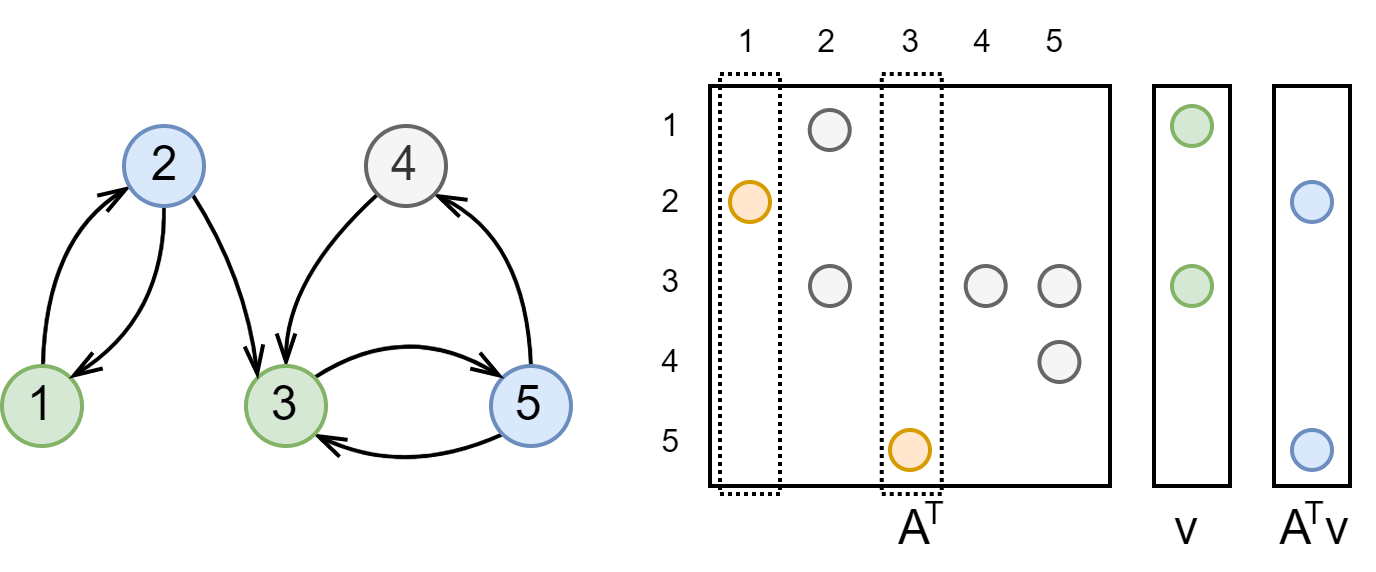
\includegraphics[width=0.9\textwidth]{images/graph_traversal_mxv.png}
    \caption{Graph traversal by matrix-vector product}
    \label{fig:gt_mxv}
\end{figure}

\subsection{GraphBLAS concepts}

GraphBLAS standard~\cite{paper:graphblas_foundations} is a mathematical notation translated into a C API. This standard provides sparse linear algebra building blocks for the implementation of graph algorithms in terms of operations over matrices and vectors. Essential parts of this standards are the following.\\

\textbf{Data containers}. Primary data containers in this standard are general M by N matrix and M vector of values, as well as a scalar value. Containers are parameterised by the type of stored elements. The standard provides a set of predefined commonly used types, as well as, the ability to declare custom user defined types. 

Matrix is used to represent the adjacency matrix of the graph. Vector is used to store a set of active vertices for traversal purposes. The scalar value is used to extract edge data from the graph or to aggregate the data across multiple edges.\\

\textbf{Algebraic structure}. Primary algebraic structures are called semiring and monoid, where two or one operation is provided respectively with some semantic requirements, such as associativity, commutativity, etc. This structures are adapted for a sparse graph analysis, so its mathematical properties differ a bit from those, which are stated in classical algebra.

These structures define the element-wise operations, which work with elements in the containers. For example, they are passed as a parameters \textit{multiply} and \textit{add} in the matrix product, where elements for row and column are multiplied, and then reduced to the final element.

There is a number of semirings, which can be used to solve different types of problems. For example, consider \textit{MinPlus} semiring $\langle min, +, \mathbb{R} \cup \{+\infty\}, +\infty \rangle$, for a shortest path problem solving, where:

\begin{itemize}
    \item Min used to aggregate distances and select the smallest one.
    \item Plus used to concatenate distances between two vertices.
    \item The domain is all real values with plus infinity.
    \item The identity element is infinity, what marks unreached vertices.
\end{itemize}

\textbf{Programming constructs}. GraphBLAS provides extra objects, which are required for practical algorithms implementation. One of these programming features is a concept of the mask. Any matrix or vector can be used as a mask, which structure defines the structure of the result. It is a crucial and essential concept, since in many cases we are interested only in a partial result, not the whole matrix or vector. Mask is passed as extra argument, and implementation is free to make the fusion of the mask into the operation.

Another important construct is a descriptor. Descriptor is a set of named parameters and associated with them values. Descriptor used to tell the implementation, that, for example, mask complementary pattern required, or result must not be accumulated with old content. This concept can be extended further, what is done in some GraphBLAS extensions.\\

\textbf{Operations.} GraphBLAS provides a number of commonly used linear algebra operations, such as matrix-vector and matrix-matrix products, transpose, element-wise multiplication. Also, there are some extra operations, which are more familiar for experienced developers, such as filtering, selection using predicate, reduction of matrix to vector or of vector to scalar, etc.

The important concept of the GraphBLAS operations is shown in the figure~\ref{fig:gb_ops}. For example, we can consider matrix-vector and matrix-matrix product operations, called \textit{mxv} and \textit{mxm} respectively. From the users perspective, they only have to use these operations, when the implementation is free to select the best algorithm, which fits the sparsity of the input arguments.\\

\begin{figure}[h]
    \centering
    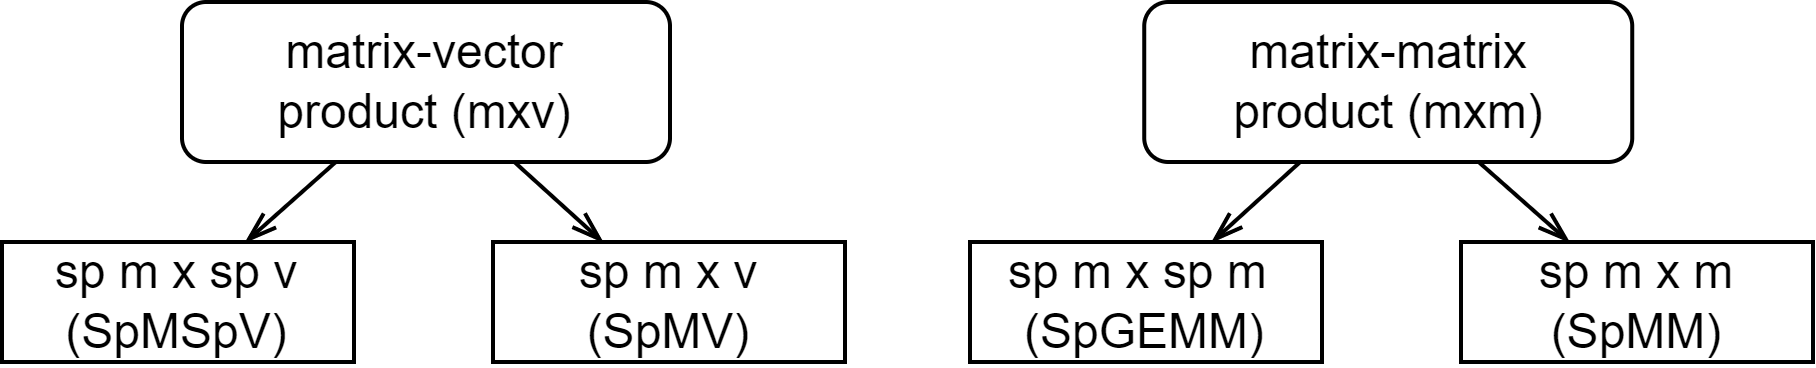
\includegraphics[width=1.0\textwidth]{images/types_of_operations.png}
    \caption{Key operations of the GraphBLAS standard and their implementations}
    \label{fig:gb_ops}
\end{figure}

\textbf{Algorithms.} Using GraphBLAS constructs it is possible to write generalized graph analysis algorithms. There is a number of common and well-known graph algorithms, such as breadth-first search (BFS), single-source shortest path (SSSP), triangles counting (TC), connected components (CC), etc. which have a linear-algebra based formulation, described by Kepner et al.~\cite{misc:la_graph}.

For example, consider a procedure with BFS algorithm in listing~\ref{alg:bfs_graphblas}. As arguments it accepts vector $v$ to store levels of reached vertices, adjacency matrix $A$, index of the start vertex $s$, and number of graph vertices $n$. Algorithm starts in lines \textbf{5 -- 9} with initialization of result vector. Also, it allocates vector $q$, which is used as a \textit{frontier} of currently active vertices to make a traversal step. The primary traversal loop in lines \textbf{14 -- 19} of the algorithm works while the frontier has at least one active vertex. In the body, it updates current traversal level. Then, it assigns current level to currently reached vertices in the frontier in line \textbf{16} using \textit{apply} function. Then in the line \textbf{17} it makes traversal step to find all children of current frontier vertices. Note, it uses inverted $v$ as a mask with \textit{GrB\_DESC\_RC} to filter our already visited vertices.

\lstset{style=codelistingstyle}

\begin{algorithm}[]
\floatname{algorithm}{Listing}
\caption{Breadth-first search using GraphBLAS API}
\label{alg:bfs_graphblas}
\begin{lstlisting}[language=C++]
#include "GraphBLAS.h"

GrB_Info BFS(GrB_Vector *v, GrB_Matrix A, GrB_Index s, GrB_Index n)
{
  GrB_Vector_new(v, GrB_INT32, n);

  GrB_Vector q;
  GrB_Vector_new(&q, GrB_BOOL, n);
  GrB_Vector_setElement(q, true, s); 

  int32_t level = 0;
  GrB_Index nvals;
  
  do {
    ++level;                                               
    GrB_apply(*v, GrB_NULL, GrB_PLUS_INT32, GrB_SECOND_INT32, q, level, GrB_NULL);       
    GrB_vxm(q, *v, GrB_NULL, GrB_LOR_LAND_SEMIRING_BOOL, q, A, GrB_DESC_RC);                           
    GrB_Vector_nvals(&nvals, q);
  } while (nvals);
  
  GrB_free(&q);

  return GrB_SUCCESS;
}
\end{lstlisting}
\end{algorithm}

\subsection{GraphBLAS limitations}

Although GraphBLAS is a mature standard with a number of implementations, it has some limitations and shortcomings, discussed in a talk given by John R. Gilbert~\cite{talk:graphblas_did_wrong}. Some of them are explained in the next paragraphs. 

\begin{enumerate}

\item \textbf{Lack of interoperability}\label{issue1}. GraphBLAS declares opaque objects with hidden from the user structure. It is not possible to some-how extend or interact with an existing standard implementation. However, some practical tasks may required integration of existing formats, storage into a library for practical tasks solving. For example, it can be use full to integrate NumPy arrays into library in order to avoid extra copy operations and reduce marshaling overhead between execution environments.

\item \textbf{Little introspection}\label{issue2}. GraphBLAS declares a very limited functionality to inspect structure, state, type, behaviour, performance, correctness, progress of library primitives and operations. It is not feasible to build production-ready data-analysis platform without featured introspection, which is a port of all modern DBMS.

\item \textbf{Implicit zeros}\label{issue3}. GraphBLAS standard tries to use a mix of math and engineering concepts to address the values storage model. As the result, this model is to complex and not obvious for both mathematicians and programmers. GraphBLAS has a know issue with a storage of implicit zeroes or identity elements in memory. Inaccurate storage manipulations may cause a sufficient memory usage increase in your application even if you correctly follow the standard.

\item \textbf{Inflexible masking}\label{issue4}. GraphBLAS standard provides an ability to apply a mask to filter out result matrices or vectors. However, rules for selecting values from a mask are implicit and rely on selecting raw zero values, like in a C program. This mechanism is not configurable. An alternative for that is the ability to select mask values using user-provided predicate.

\item \textbf{Templates usage}\label{issue5}. There is a number of libraries which implement GraphBLAS in a form of C++ interface. These libraries heavily rely on a template meta programming for a generalization of a processed data. This approach simplifies implementation of the library, reduce number of auxiliary code (in this case, it is generated by the compiler). However, template based approach requires the whole project recompilation for each executable and for any change of a source code. Distribution of a such solution cannot be done in a form of binary file, since the user must compile the library locally each time for usage.

\item \textbf{GPU support}\label{issue6}. GraphBLAS has no fully-featured implementation with GPU support. The primary reason for this is the complexity of the standard. There is a number of attempts to adopt GraphBLAS for a GPU analysis. But, most of them are focused only on Nvidia platform, what limits the portability of the potential solution.

\end{enumerate}

Summarizing, the GraphBLAS is solid and mature standard with a number of some conceptual and technical shortcomings. Thus, it is important to overcome these technical limitations and address some conceptual problems designing similar yet distinct API, which can be wrapped with GraphBLAS API if required.

\subsection{GPU computations}

\textit{GPGPU} (general-purpose computing on graphics processing units) is a technique of graphics processor utilization of a graphics card accelerator for a non-specific computations, which are typically done by a central processing unit of a computer. This technique allows to get a \textit{significant} speedup, when the computation involve large homogeneous data processing with a fixes set of instructions.

There is a number of existing industry standards for a development of GPU programs, such as Vulkan, OpenGL, DirectX, Metal for graphics and computations tasks, as well as OpenCL, SyCL, Nvidia Cuda for computational tasks only.

Existing graph analysis tools in most cases use OpenCL and Nvidia Cuda APIs for GPU work offload. The following sections provide a brief overview for each of this technologies.\\

\textbf{Nvidia Cuda}. It is an industrial proprietary technology, created by a Nvidia, which is available on graphics devices of this vendor only. This API has rich language support for C and C++ programs. It supports template meta programming, what allows to implement generalized parallel GPU algorithms, such as \textit{sort}, \textit{scan}, \textit{reduce}, which are parameterized by the type of sorted element and used functions and predicates. Also, Nvidia provides a rich set of tools of debugging and profiling Cuda code. What simplifies development significantly.\\

\textbf{OpenCL}. It is an open industrial standard for a programs' development, which utilize different accelerators for parallel computations. This standard is supported on a number of platforms, such as Nvidia, AMD, Intel, Apple M1, what makes it portable for usage on a large spectrum of devices. This API is designed in a form of C interface. It doesn't have built-in support for generalized meta-programming (opposite to Cuda support). Since this is an open standard, its supports varies significantly from platform to platform. What makes the development and testing of OpenCL application as a complex tasks.\\

\textbf{SyCL}. It is a higher-level programming model to improve programming productivity on various hardware accelerators. It is a single-source embedded domain-specific language based on pure C++ standard language. The SyCL is a open-source standard maintained by a Khronos Group. SyCL allows to program heterogeneous computations within single C++ application, while the compiler infrastructure is used to translate SyCL specifics into specific computations backend. This is a new and promising technology, while its support across different compilers, devices and operating systems is still debatable.\\

In this work the OpenCL is utilized as a API for GPU computations. This API is chosen, since its required for the project version 1.2 is supported on all actual devices. OpenCL API is low-level. It gives precise control over execution and resources management. Also, this API allows dynamic code compilation in runtime for GPU execution. What makes it is usable for creating generalized library, where the user is able to implement custom primitive types and operations in a form of OpenCL code, passed as a string.

\subsection{GPU architecture}

This section gives an overview for a typical GPU architecture. Understanding of a target hardware is a key to performance optimizations, required to speed up developed GPU library.

The particular GPU architecture is a very controversial topic for a discussion. Implementation details of a given GPU depend on a number of factors, such a GPU's vendor, family, generation, etc. Thus, writing an efficient GPU code forces a programmer to learn a particular details of a target processor for execution. For the sake of brevity, let's focus on an existing, open-source and well-document state-of-the-art modern GPU microarchitecture such as AMD's RNDA.

Radeon DNA (RDNA) is a GPU microarchitecture and accompanying instructions set architecture developed by AMD. The block diagram of Radeon RX 5700 XT GPU having RDNA architecture is depicted in a figure~\ref{fig:rdna_gpu}. The GPU itself is placed on a infinity fabric surface for a fast data interconnect between units. PCIe controller allows communication of a GPU with the system RAM. 

\begin{figure}
    \centering
    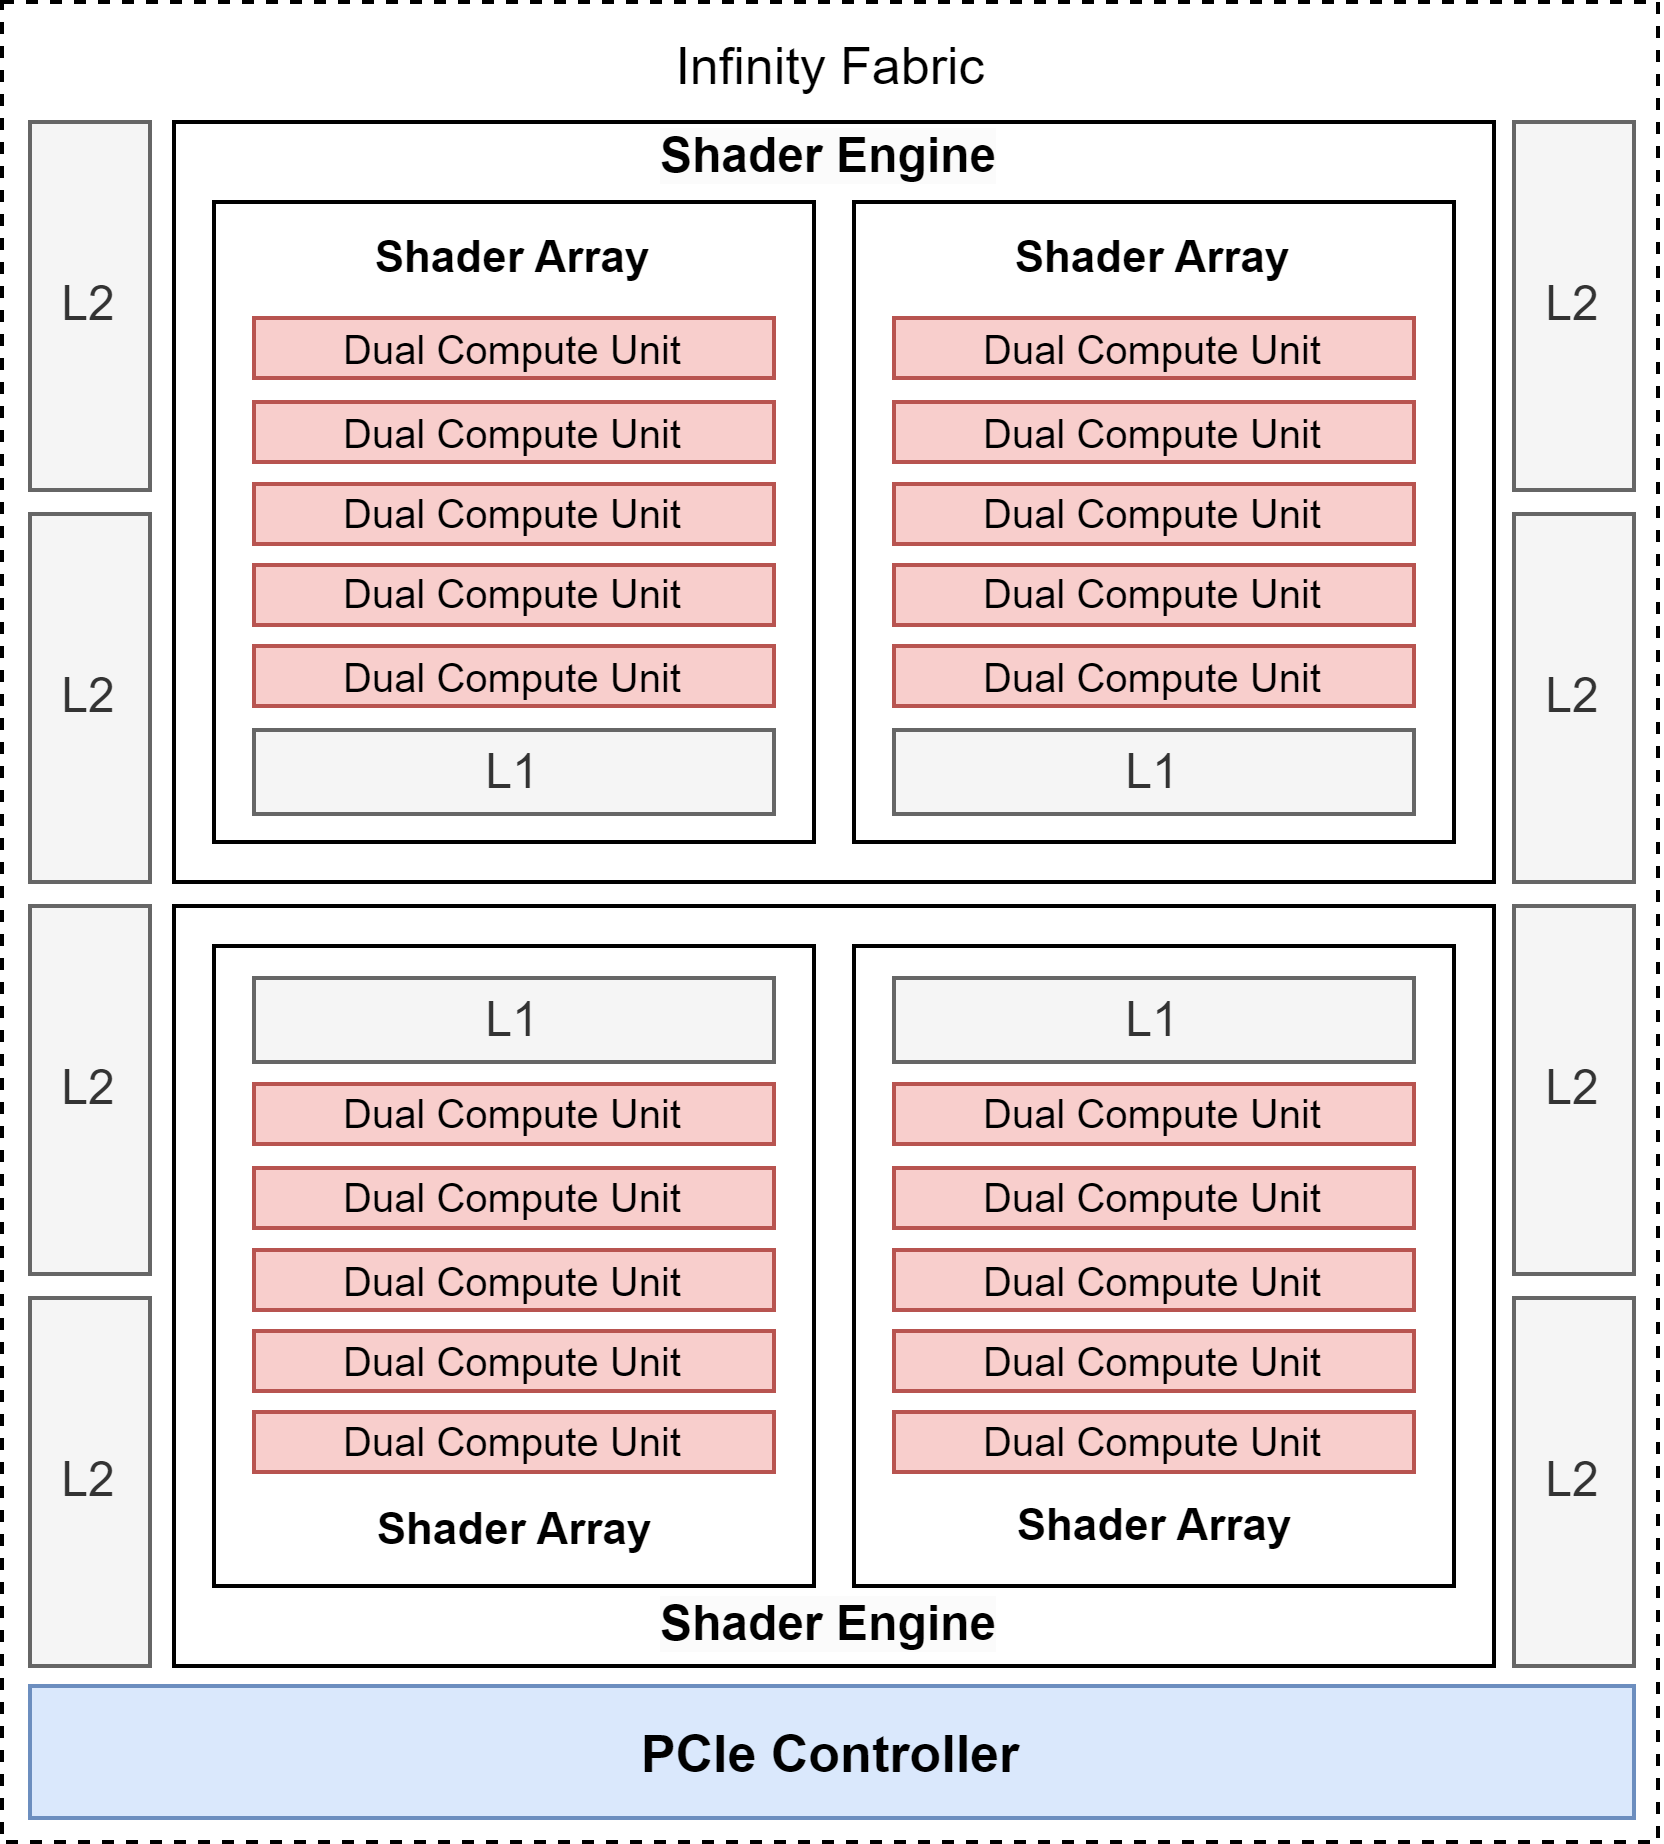
\includegraphics[width=1.0\textwidth]{images/rdna_gpu.png}
    \caption{The block diagram of a Radeon RX 5700 XT GPU powered by the RDNA architecture.}
    \label{fig:rdna_gpu}
\end{figure}

The GPU is composed of two \textit{shader engines}. Each engine has a number of \textit{shader arrays}. Each array possess own L1 cache and a set of actual \textit{dual compute units}, which responsible for computation work. Shader engines surrounded by a L2 shared cache. Any of L2 banks can be accessed by shader array during the computations.

Programs for the execution are structured in a form of \textit{kernels}. Kernel is a single stream of instructions that operate on large number of data parallel work items. The work items organized into a work grouts, which can communicate explicitly through local memory. The shader compiler sub-divides the work groups further into micro-architecture specific wavefronts that are scheduled for parallel execution on a compute unit.

\begin{figure}[h]
    \centering
    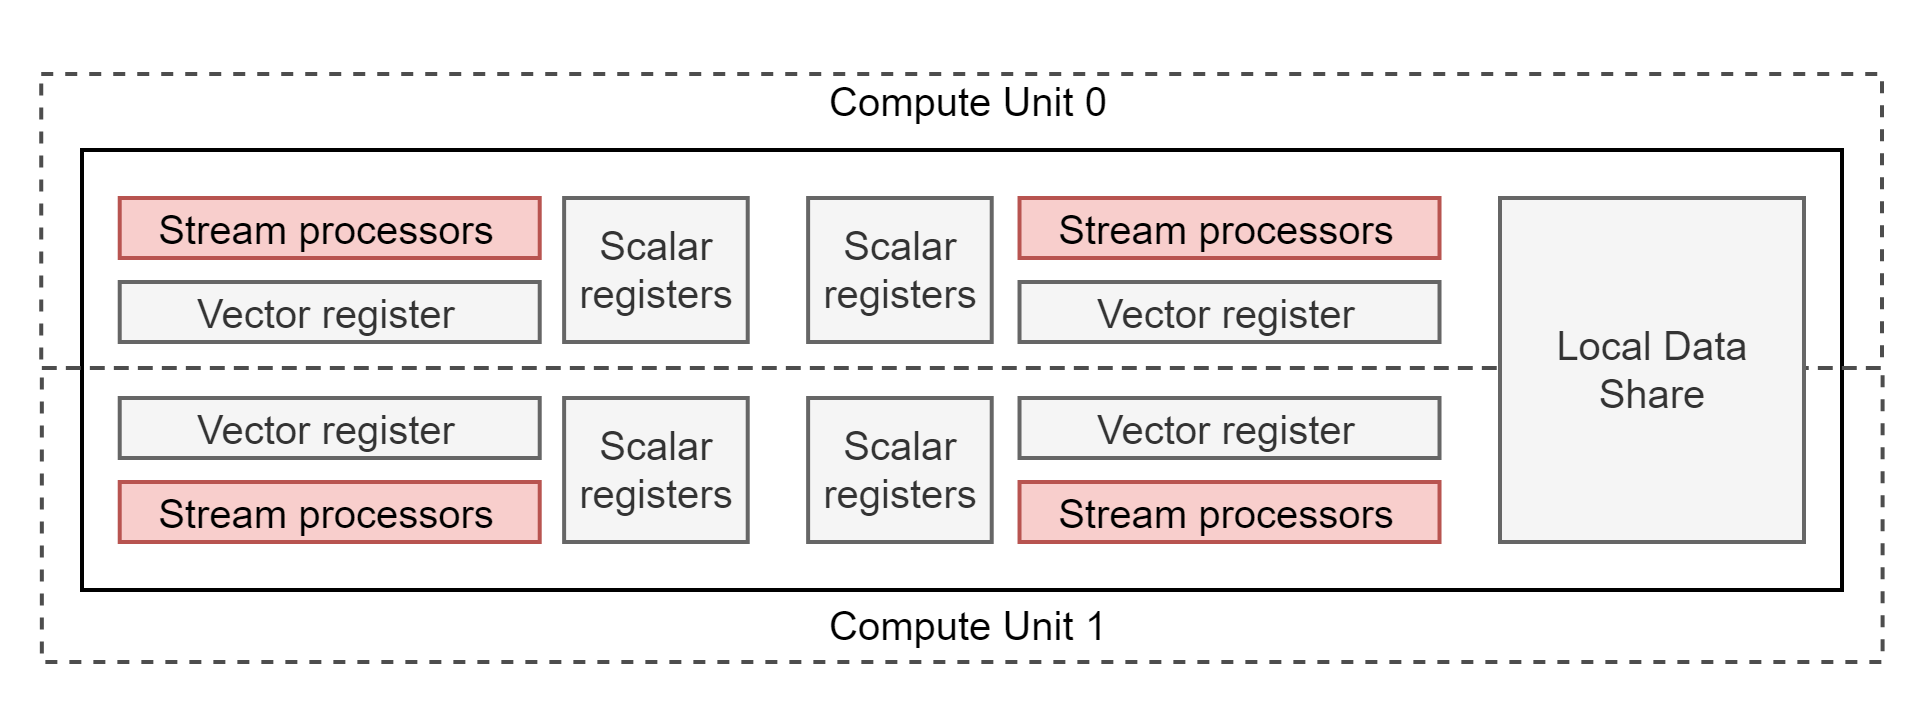
\includegraphics[width=1.0\textwidth]{images/rdna_dcu.png}
    \caption{AMD Radeon DNA dual compute unit. Compute unit consist of a number of SIMD processors. Each processor has independent registers set. All processors share local memory, called local data share in AMD terms.}
    \label{fig:rdna_dcu}
\end{figure}

Dual compute unit in AMD architecture is depicted in a figure~\ref{fig:rdna_dcu}. Compiler crates wavefronts of a size 32 (wave32). Every item inside a wavefront is executing the same instruction (SIMD). Each compute unit (CU) includes four SIMD units. Each SIMD unit has 32 ALUs, has 32-wide vector registers and scalar registers. SIMD executes full wavefront instruction over single clock cycle.

Thus, writing an OpenCL kernel requires saturation of CU with works as well as keeping all slots of a SIMD processor active. Elimination of some of these features causes inefficiency and, as the consequences, performance drop of a target application.

\subsection{OpenCL concepts}

This section gives a brief introduction to the OpenCL standard. This section covers platform, execution and memory model. It introduces essential programming constructs and gives and understanding on how a typical OpenCL program is written.\\

\textbf{Platform}. OpenCL exists in a context of a platform. Platform in OpenCL terms is vendor, or organization, which provides OpenCL implementation for a target machine. Several platforms on single machine may be available. It depends on the installed CPU, GPU or FPGA. 

Typical providers of OpenCL implementations are Intel, Nvidia, AMD and Apple. For computations only single platform can be selected. Thus, resources and features are not shared between different implementations.

OpenCL is an open API. Its implementation and support is optional. So, the presence of the OpenCL, actual version, set of features and extensions is a subject, which varies a lot from one system to another.\\

\textbf{Execution}. Execution of an OpenCL program takes within an execution context. Context is an environment, which is created using platform and list of devices, which must be used for computations. Context keeps track of all resources, manages global execution state.

Device is an logical unit, which performs operations. Several devices may be available in a single platform. Typical devices are integrated Intel GPUs, discrete Nvidia or AMD video adapters.

Device consists of a set of compute units. Compute unit is a small processor with its own instruction and data caches, registers, controllers. Distinct compute units can run distinct programs. However, single compute unit can run only single program at given time.

Work for a compute unit is structured as work items. Single work item inherently is a thread, which executes instructions stream and has own registers.\\

\textbf{Memory}. The whole available memory for an OpenCL program is divided into three parts. Global memory is available across all devices within a context. In most cases, it is a dedicated VRAM with L2 cache of the GPU. Local memory is a memory available only within single compute unit. This memory is visible only inside this unit. It is not persistent, and exist only in time or program execution. Local memory is registers, available for a single work item.\\

\textbf{Programming}. OpenCL provides C-compatible API for applications development. From a user point of view an OpenCL program is a set of kernel invocations with some resources, bound to the kernel. 

Resources are different memory buffers or textures, which can be consumed on a GPU for read/write operations. These resources created from CPU side using specialized C API. The data inside buffers can be access using copy commands or specialized map/unmap functions. Actual location for a storage is hidden for the user. However, it is possible to hint storage properties using some flags.

Kernels are scheduled for the execution using command queues. Command queue is an logical abstraction, which control the order of execution of different kernels. User can create multiple command queues and synchronize them using specialized events. Commands queues mapped to hardware queues automatically by the OpenCL driver.

Kernel is a special function, written using C-language extension and compiled using OpenCL built-in compiler. This function is invoked for each work item to perform some meaningful work.\\

\subsection{Implementation challenges on GPUs}

GPU programming in a connection with a sparse linear algebra domain and large data processing introduces an number of challenges, which must be addressed by the developers of a such frameworks.\\

\textbf{Fine-grained parallelism}. The most straightforward method of a parallelism is a vertex-based parallelism. However, in many graph, particularly scale-free graphs, the number of outgoing edges per vertex may vary dramatically. In this case, the time of processing of such a vertex will vary in the same way. Thus, assigning a tread per vertex will cause a significant load imbalance in a such case. 

This problem may scale to sparse linear algebra approach, where a row of a matrix can be assigned per a thread. So, it is important to dynamically define the load balance and assign different number of threads, accounting the possible amount of work to occur.\\

\textbf{Minimizing overhead}. GPU kernels running on a large load balanced dataset with a large number of computations achieve the maximum throughput. However, in some cases, the runtime may be dominated by the overhead, not by a computations. For example, GPU kernel may do not have enough work to occupy the whole computational device. In this case, many GPU processing block will be stalled and unused. 

Synchronization points can also introduce additional overhead. GPU cores will finish their work and be stalled until the synchronization point is reached. Only after this point the new work will be offloaded. Also, one of the possible overheads may be introduced by the driver runtime. JIT GPU kernels compilation, data transfer to GPU and kernel launch may take additional time.\\

\textbf{Computations intensity}. Good GPU kernel may be characterised as highly parallel grid of threads, where each group of threads process a small portion of the data, which must fit into the on-chip L1 memory. In this case the peak performance is achieved, since the memory latency is minimized to its limits. However, it is almost never achieved in a graph processing kernels, where the working threads have a lot of unstructured memory load operations with pure computational work, which cannot be avoided.\\
